\documentclass[10pt]{article}
\usepackage[sc]{mathpazo}
\usepackage{commands}

\let\oldphi\phi 
\let\phi\varphi 
\let\varphi\oldphi





\begin{document}

\begin{figure}[h!]
	\centering
	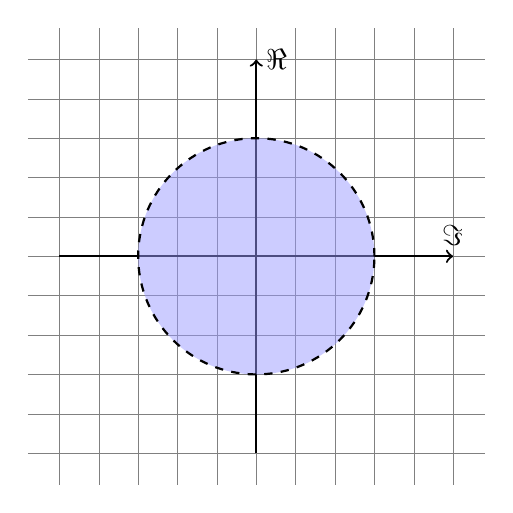
\begin{tikzpicture}
		\draw[step=0.5, black!10!white, help lines](-2.9,-2.9) grid (2.9, 2.9);
		\draw[thick, ->] (-2.5,0) -- (2.5,0) node[anchor=south] {$\Im$};
		\draw[thick, ->] (0,-2.5) -- (0,2.5) node[anchor=west]{$\Re$};
		\filldraw[blue!40!white, thick, dashed, draw=black, fill opacity=0.5] (0,0) circle (1.5cm);
	\end{tikzpicture}
	\caption{The planar set representing $ |z| \le 3 $}
\end{figure}



\begin{figure}[h!]
	\centering
	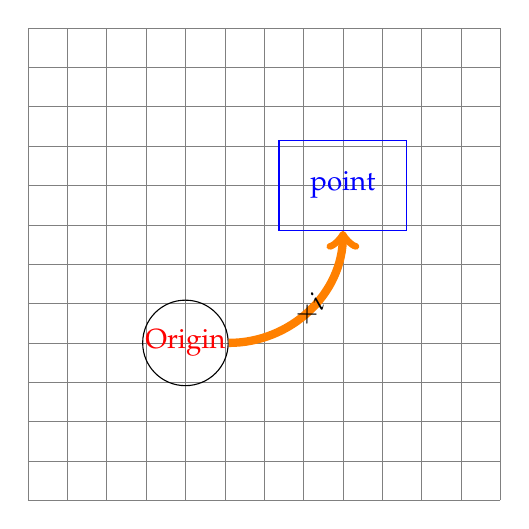
\begin{tikzpicture}[inner sep=4mm]
		\draw [step=0.5, gray, very thin] (-2,-2) grid (4,4);
		\coordinate (O) at (0,0);
		\coordinate (A) at (2,2);
		\node[red, circle, draw=black,inner sep=0.1] (P1) at (O) {Origin};
		\node[blue, rectangle, draw] (P2) at (A) {point};
%		\path (O) node[circle,draw](O) {Origin} (A) node[circle,draw](A) {h};
		\draw[->,orange,line width=3] (P1) to[out=0, in=-90] node[pos=0.5,sloped,black]{$\times i$} (P2);

	\end{tikzpicture}
	\caption{Practicing with nodes}
\end{figure}


\begin{figure}[h!]
	\centering
	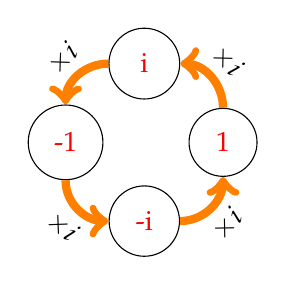
\begin{tikzpicture}[inner sep=4mm]
%		\draw [step=0.5, gray!50!white, line width=0.1] (-2,-2) grid (2,2);
		\node[red, circle, draw=black,inner sep=0.2cm] (1) at (1,0) {1};
		\node[red, circle, draw=black,inner sep=0.23cm] (i) at (0,1) {i};
		\node[red, circle, draw=black,inner sep=0.2cm] (-1) at (-1,0) {-1};
		\node[red, circle, draw=black,inner sep=0.2cm] (-i) at (0,-1) {-i};
		\draw[->, orange, line width=3] (1) to[out=90, in=0] node[sloped, black, anchor=south,inner sep=1mm] {$\times i$} (i);
		\draw[->, orange, line width=3] (i) to[out=-180, in=90] node[sloped, black, anchor=south,inner sep=1mm] {$\times i$} (-1);
		\draw[->, orange, line width=3] (-1) to[out=-90, in=180] node[sloped, black, anchor=north,inner sep=1mm] {$\times i$} (-i);
		\draw[->, orange, line width=3] (-i) to[out=0, in=-90] node[sloped, black, anchor=north,inner sep=1mm] {$\times i$} (1);
%										
%										;

		
	\end{tikzpicture}
	\caption{Practicing with nodes}
\end{figure}

\end{document}